\section{Additional experimental details} \label{app:additional_experimental_results}

\subsection{Experimental Setup} \label{app:additional_experimental_results:experimental_details}

Our experimental analysis of \umup\ was conducted by adapting the codebase used for Tensor Programs V, allowing us to compare \mup\ and \umup\ in the same setting. We change various experimental settings from the original paper to make our experiments better reflect standard training procedures, particularly the dataset which we switch from WikiText-2 to the larger WikiText-103 \citep{WikiText103}. Where not specified otherwise, the default setting used in our experiments are given in \Cref{tab:experiment_defaults}. These also represent the settings of our proxy model.

\begin{table}[h] 
    \centering
    \renewcommand{\arraystretch}{1.25}
    \begin{tabular}{|r|p{10cm}|}
    \hline
        Dataset & WikiText-103 \citep{WikiText103} \\
        Sequence length & $256$ \\
        Vocab size & $32000$ \\
        Training set tokens & $138\mathrm{M}$ \\
        \hline
        Architecture & Llama \citep{Llama} \; (Transformer, PreNorm, RMSNorm, SwiGLU, RoPE, ``untied'' embeddings), non-trainable RMSNorm parameters. \\
        Width & $256$ \; (scaled up to $4096$) \\
        Depth & $4$ \\
        Number of heads & $4$ \; (scaled up to $64$) \\
        Head dimension & $64$ \\
        Total parameters & $19.5M$ \; (scaled up to $1.07\mathrm{B}$)\\
        \hline
        Batch size & $64$ \\
        Training steps & $8192$ ($0.97$ epochs) \\
        LR schedule & Cosine to $10\%$, $2000$ steps warm-up \\
        Optimizer & AdamW $(\beta_1, \beta_2, \epsilon) = (0.9, 0.999, 10^{-8})$ \\
        Weight decay & $2^{-13}$, independent \citep{Independent_WD} \\
        Dropout & $0.0$ \\
        \hline
         \mup{} HP search range &
        $\eta \in [2^{-10}, 2^{-6}]$\\
        &$\hat{\eta}_{\mathrm{emb}} \in [2^{0}, 2^{8}]$\\
        &$\sigma_{\mathrm{init}},
        \alpha_{\mathrm{emb}},
        \alpha_\mathrm{{attn}},
        \alpha_{\mathrm{output}} \in [2^{-2}, 2^{2}]$\\
        \umup{} HP search range &
        $\eta \in [2^{-1}, 2^{3}]$\\
        &$\alpha_{\mathrm{attn}} \in [2^{-2}, 2^{2}]$\\
        &$\alpha_{\mathrm{residual}},\alpha_{\mathrm{residual{\text -}attn{\text -}ratio}},\alpha_{\mathrm{ffn{\text -}act}},\alpha_{\mathrm{output}} \in [2^{-3}, 2^{3}]$\\
         \hline
        \mup{} HP defaults &
        $\sigma_{\mathrm{init}}=
        \alpha_{\mathrm{emb}}=
        \alpha_\mathrm{{attn}}=
        \alpha_{\mathrm{output}}=
        \hat{\eta}_{\mathrm{emb}}=1$\\
        \umup{} HP defaults &
        $\alpha_{\mathrm{residual}}=
        \alpha_{\mathrm{residual{\text -}attn{\text -}ratio}}=
        \alpha_{\mathrm{ffn{\text -}act}}=
        \alpha_{\mathrm{output}}=
        \alpha_{\mathrm{attn}}=1$\\
    \hline
    \end{tabular}
    \caption{Default hyperparameters and training settings.}
    \label{tab:experiment_defaults}
\end{table}

\FloatBarrier
\clearpage

\subsection{Per-tensor learning rates}\label{app:umup_lr_mults}

In \Cref{sec:umup:principled_hps} we relax the requirement for each weight tensor in the \umup\ model to have an associated tuneable learning-rate multiplier on top of the global learning rate. Whilst this does reduce the theoretical expressivity of the \umup\ scheme, \Cref{fig:additional_experiments:lr_mults} shows that using a single globally optimized learning rate is already at or close to the optimal choice for all weight tensors, and therefore it is reasonable to drop these multipliers in favor of reducing the number of HPs. However, a practitioner attempting to absolutely maximize the task performance of their model could experiment with tuning a few key per-tensor LRs, in particular the embedding table.

\begin{figure}[h]
    \centering
    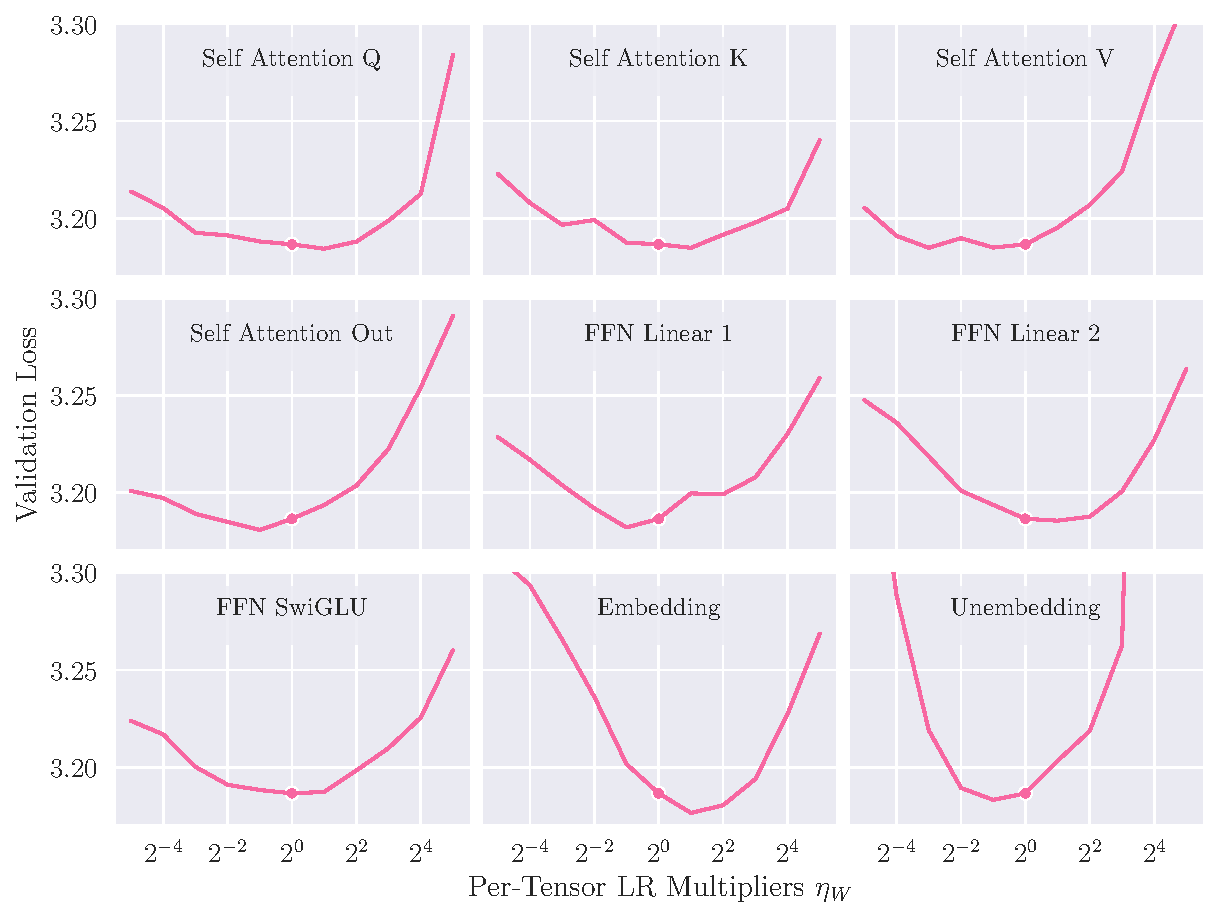
\includegraphics[width=\textwidth]{arXiv/figures/fig_LR_mults.pdf}
    \caption{Independently varying per-tensor learning rate multipliers $\eta_W$, using the \umup\ model of width 256 from \Cref{fig:fig1} with optimized global learning rate $2^{1.5}$ as the starting point. Where applicable, the same multiplier is used for tensors of the same name across transformer layers. Each subplot fixes all but one multiplier at 1, therefore the midpoint of each subplot is precisely the \umup{}$_{256}$ model from \Cref{fig:fig1}.}
    \label{fig:additional_experiments:lr_mults}
\end{figure}

\subsection{Hyperparameter independence}

In \Cref{sec:experiments:hp_independence} we explore the question of HP independence under \mup\ and \umup. The following plots in \Cref{fig:additional_experiments:mult_grid_mup,,fig:additional_experiments:mult_grid_umup} show the result of a 2D sweep over every pair of HPs under each scheme. All other HPs are held at 1 when not swept, except the $\eta$ which is held at $2^{-7.5}$ for \mup\ and $2^{1.5}$ for \umup, and $\hat{\eta}_\mathrm{emb}$ which is held at $2^4$ for \mup.

These results show visual dependence between \mup\ hyperparameters as a diagonal structure in the grids, such as $(\hat{\eta}_{\mathrm{emb}}, \sigma_{\mathrm{init}})$ and $(\eta, \alpha_{\mathrm{attn}})$. We quantify this in the plot in \Cref{fig:experiments:transfer_error}, where we use a measure of HP dependence termed transfer error. This is explained verbally in \Cref{sec:experiments:hp_independence}, and we provide an algorithmic description in \Cref{alg:transfer_error}. We note that differences in transfer error between the two methods may also be influenced by the flatness of the optimum. The HP and loss values used for our transfer error calculations are those in \Cref{fig:additional_experiments:mult_grid_mup,,fig:additional_experiments:mult_grid_umup}.

\begin{figure}[h]
    \centering
    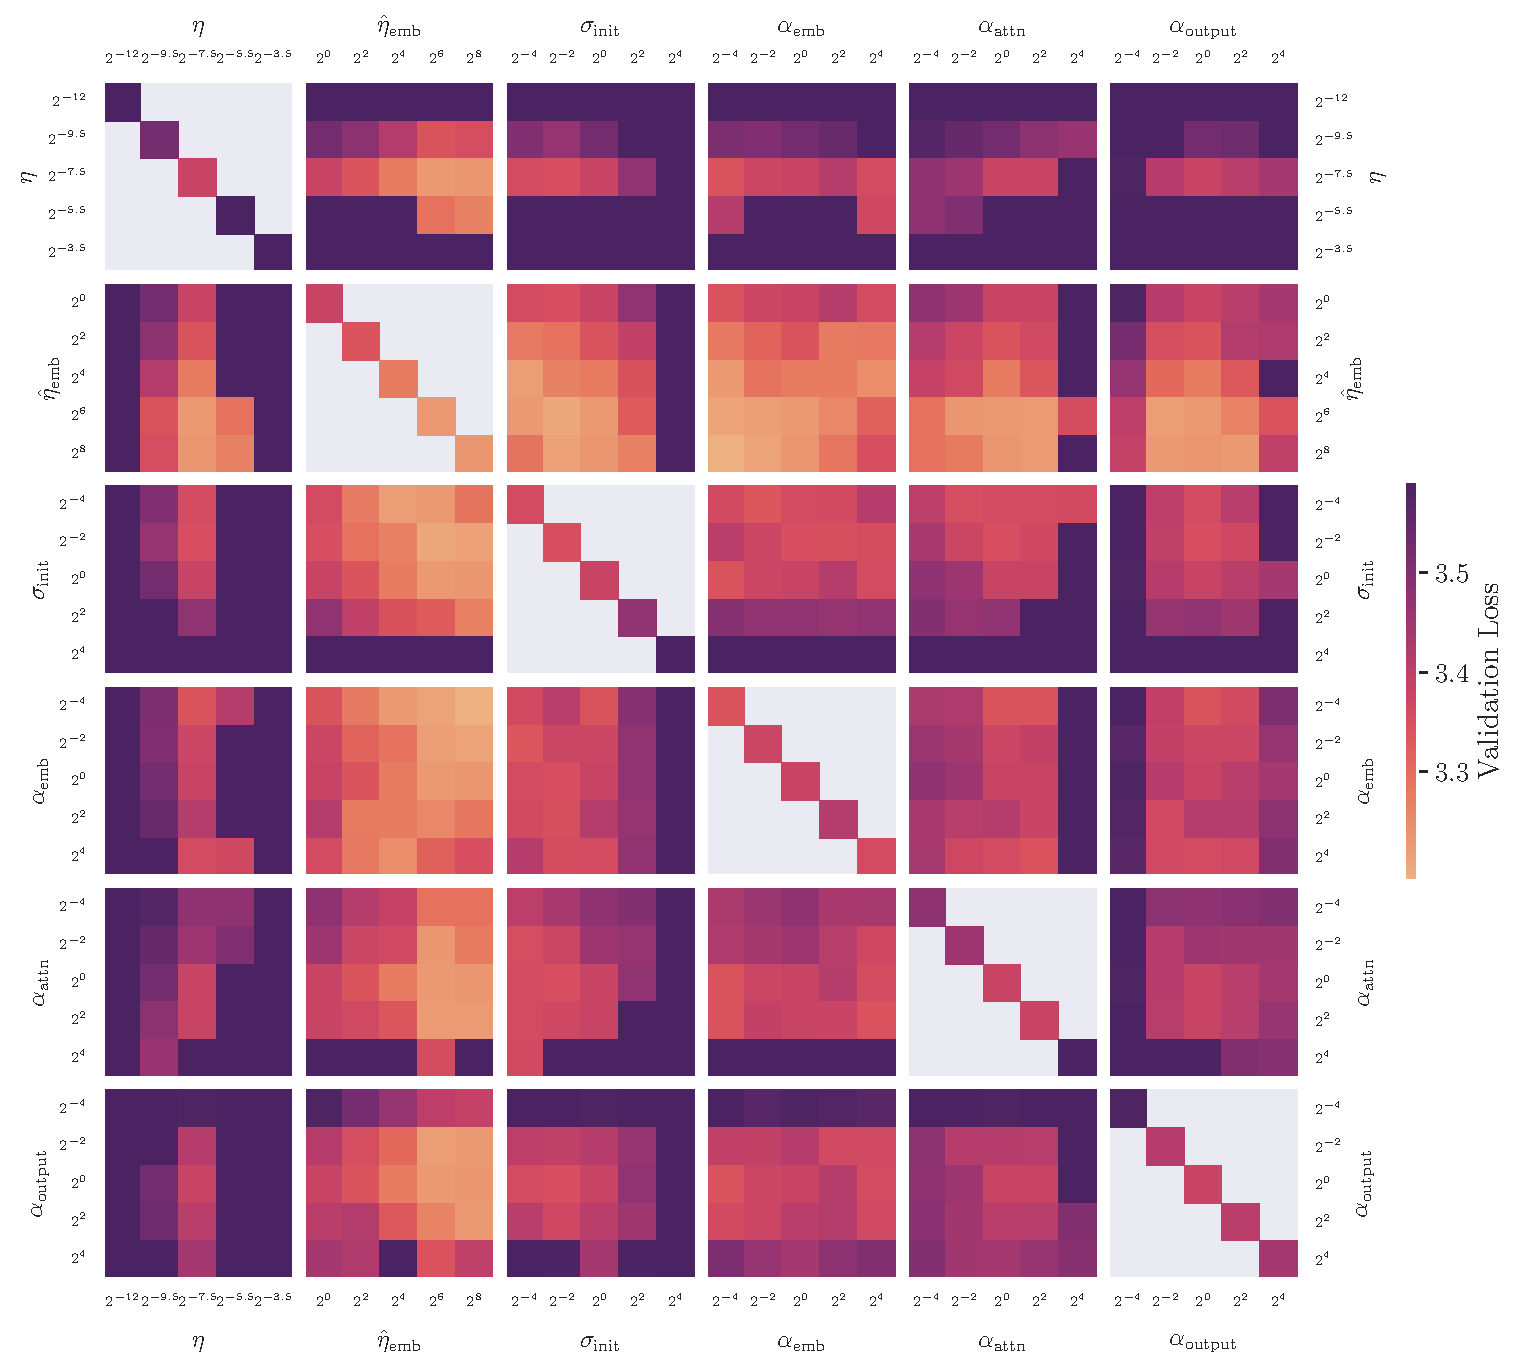
\includegraphics[width=\textwidth]{arXiv/figures/mult_grid_mup_val.pdf}
    \caption{Hyperparameter coupling sweep for \mup{}. Note strong coupling between optima, e.g. in the cases of $(\hat{\eta}_{\mathrm{emb}}, \sigma_{\mathrm{init}})$ and $(\eta, \alpha_{\mathrm{attn}})$. See also: \umup{}, \Cref{fig:additional_experiments:mult_grid_umup}.}
    \label{fig:additional_experiments:mult_grid_mup}
\end{figure}

\begin{figure}[h]
    \centering
    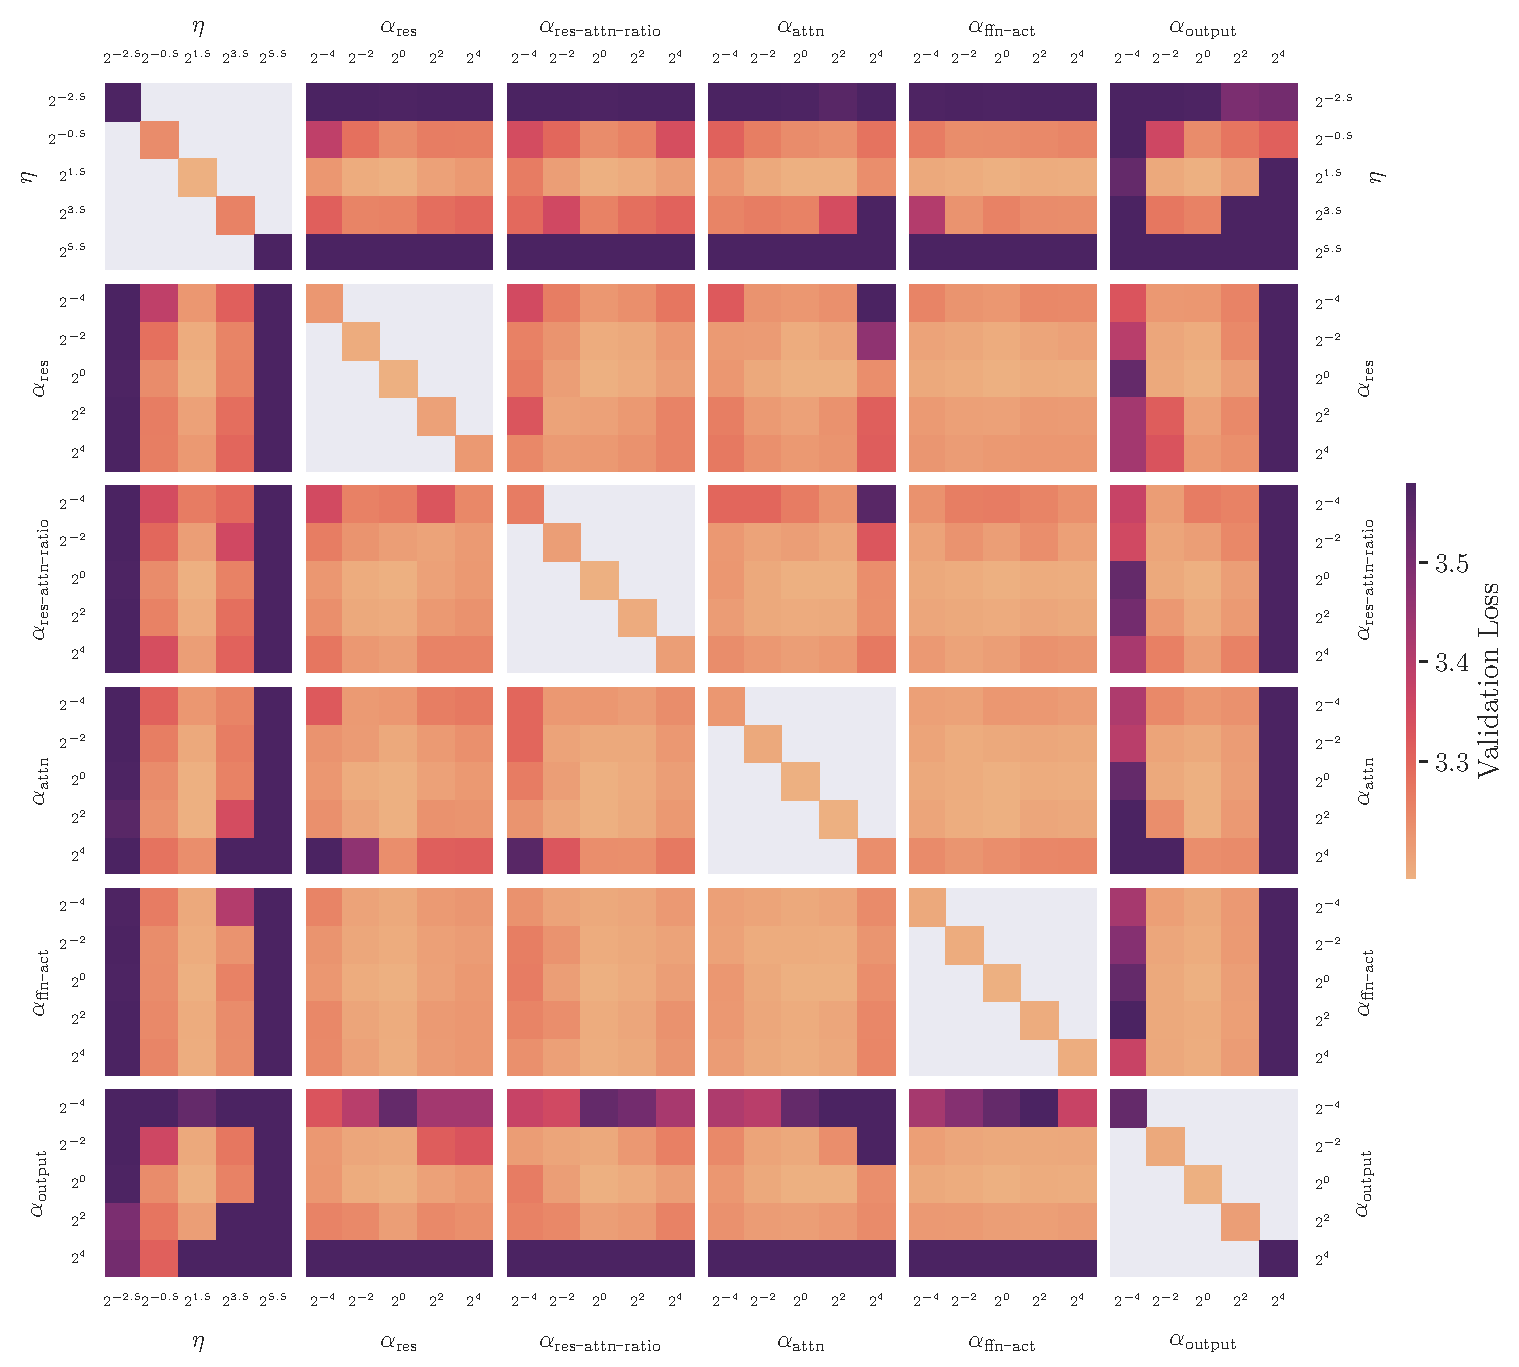
\includegraphics[width=\textwidth]{arXiv/figures/mult_grid_u-mup_val.pdf}
    \caption{Hyperparameter coupling sweep for \umup{}. Note less coupling than with \mup{}, see \Cref{fig:additional_experiments:mult_grid_mup}.}
    \label{fig:additional_experiments:mult_grid_umup}
\end{figure}

\begin{algorithm}
\caption{Transfer Error} \label{alg:transfer_error}
\begin{algorithmic}
\Require A `fixed' HP with candidate values $F = \{f_1, \cdots, f_n\}$,
a `transfer' HP with candidate values $T = \{t_1, \cdots, t_m\}$, a function that gives the final validation loss for the pair of HPs $L : F \times T \to \mathbb{R}$ (assuming all other HPs are fixed at default values).
\\
\State $\mathrm{err} \gets 0$
\State $f^*, t^* \gets \operatorname{argmin}(L)$
\For{$f$ in $F$}
    \If{$f \neq f^*$}
        \State $t \gets \operatorname{argmin}(L(f))$
        \State $\mathrm{err} \mathrel{+}= L(f^*, t) - L(f^*, t^*)$
    \EndIf
\EndFor
\\
\Return $\mathrm{err}/ (n - 1)$
\end{algorithmic}
\end{algorithm}

\FloatBarrier
\clearpage

\subsection{Hyperparameter search} \label{app:umup_hp_search_algorithm}

Here we outline the particular search processes used for our \mup\ and \umup\ HP sweeps in \Cref{fig:fig1}~(a). The \textit{random search} samples uniformly from a grid defined over all \textit{extended} HPs (extended HP sets are defined in \Cref{table:hp_sets}, with grid values defined in \Cref{tab:experiment_defaults}). We perform the random search over 339 runs, each of which is a full training of the width-256 proxy model. We then simulate the effect of shorter searches at various run-counts by taking a random sample of the results, resulting in the smooth curve over run-count shown.

The \textit{independent search} consists of the following phases:

\begin{enumerate}
    \item Perform a 1D line search for an optimal learning rate, with other hyperparameters set to their default values ($9$ runs).
    \item For each hyperparameter in parallel, perform a 1D line search ($330$ runs).
    \item Combine the best settings from step 2, and re-evaluate ($6$ runs).
\end{enumerate}

The number of runs in the 1D line search is an order of magnitude higher than is required in practice. We do so to form a fair comparison with the random search, which benefits from this large number of runs. The number of runs for the 1D line search could be reduced further by using binary search, though this would require sequential runs and limit the extent of parallelism.

\FloatBarrier

\subsection{Hyperparameter transfer experiments} \label{app:transfer_experiments}

\paragraph{LR transfer over width} The transfer experiments shown in \Cref{fig:fig1} (b) use the non-LR HPs found in \Cref{fig:fig1} (a) (indicated by the circled points), rather than using default HP values. For the \umup\ sweep we take the HPs at the end of the LR portion of the independent search, as these are already close-to-optimal, and means only 9 runs were required in the sweep. In contrast, for \mup\ it is necessary to use the results of the random search over a large number of runs.

\paragraph{LR transfer over other axes} For the training steps, batch size and depth transfer experiments in \Cref{fig:lr_transfer}, all HP values are fixed to 1 except LR which is swept. As with width transfer, \umup\ outperforms \mup\ here using these default HP values. Reducing training steps is done by fixing the number of warm-up steps (at 2000) and still cosine-decaying the learning rate to $10\%$; all that changes is the number of post-warm-up steps. We found this to be more effective than cutting-short the decay schedule.
For both \Cref{fig:fig1} (b) and \Cref{fig:lr_transfer} we sweep the LR over a logarithmically-spaced grid of step $2^{1/2} \times$, with 3 runs for each point.

Additionally, in \Cref{fig:additional_experiments:lr_transfer_over_seqlen} we show learning rate transfer over sequence length for both \mup\ and \umup\, fixing either tokens per batch or sequences per batch. In both scenarios \umup\ shows not only better absolute training performance, but also better transfer behaviour as sequence length increases. Since our default proxy sequence length is 256, using \mup\ to transfer to sequence length 2048 would result in minimal improvements or even a degradation in validation loss, whereas the \umup\ shows much greater and more consistent improvements.  

\begin{figure}[h]
    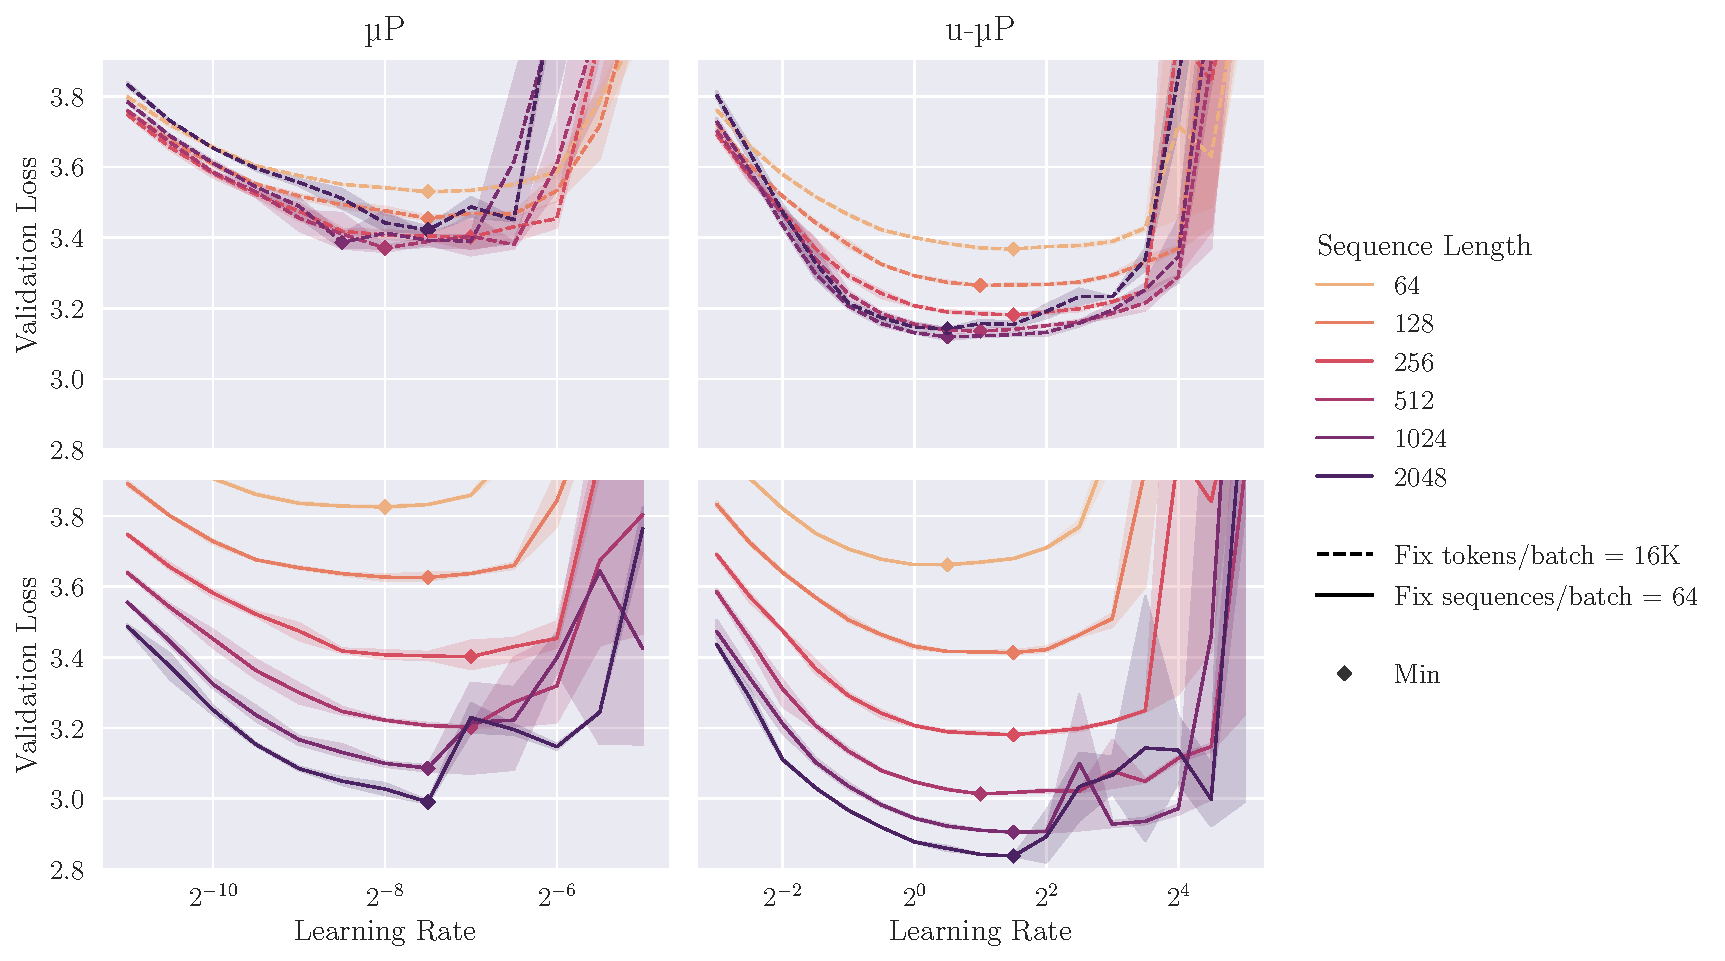
\includegraphics[width=\textwidth]{arXiv/figures/seqlen_transfer.pdf}
    \caption{Transfer of learning rate over sequence length for \mup{} (left) and \umup{} (right). As sequence length varies, we can fix the number of tokens per batch by inversely varying the number of sequences per batch (top). Alternatively we can fix the sequences per batch and allow the number of tokens per batch to vary with sequence length (bottom). In the latter case, larger sequence lengths mean the model sees more tokens during training, though as per \Cref{tab:experiment_defaults} this translates to >1 epoch on WikiText-103 when sequence length goes above 256.}
    \label{fig:additional_experiments:lr_transfer_over_seqlen}
\end{figure}

\paragraph{Other HP transfer over width} For our non-LR HP transfer results in \Cref{fig:experiments:hp_transfer_over_width}, we note that good transfer under \mup\ has not been demonstrated for all HPs used in the literature. This is particularly true for the $\hat{\eta}_\mathrm{emb}$ HP, which has poor transfer under \mup. Our investigation here led to our identification of the need to adjust the embedding LR scaling rule outlined in \Cref{sec:umup:emb_lr_rule}. In many cases users have not swept this HP, but instead swept the corresponding parameter multiplier $\alpha_\mathrm{emb}$. How this HP interacts with the embedding LR scaling problem identified (and our proposed fix) remains to be explored, though we note in \Cref{fig:experiments:hp_transfer_over_width} that it also appears to have poor transfer.

\begin{figure}[h]
    \centering
    \begin{subfigure}{\textwidth}
        \centering
        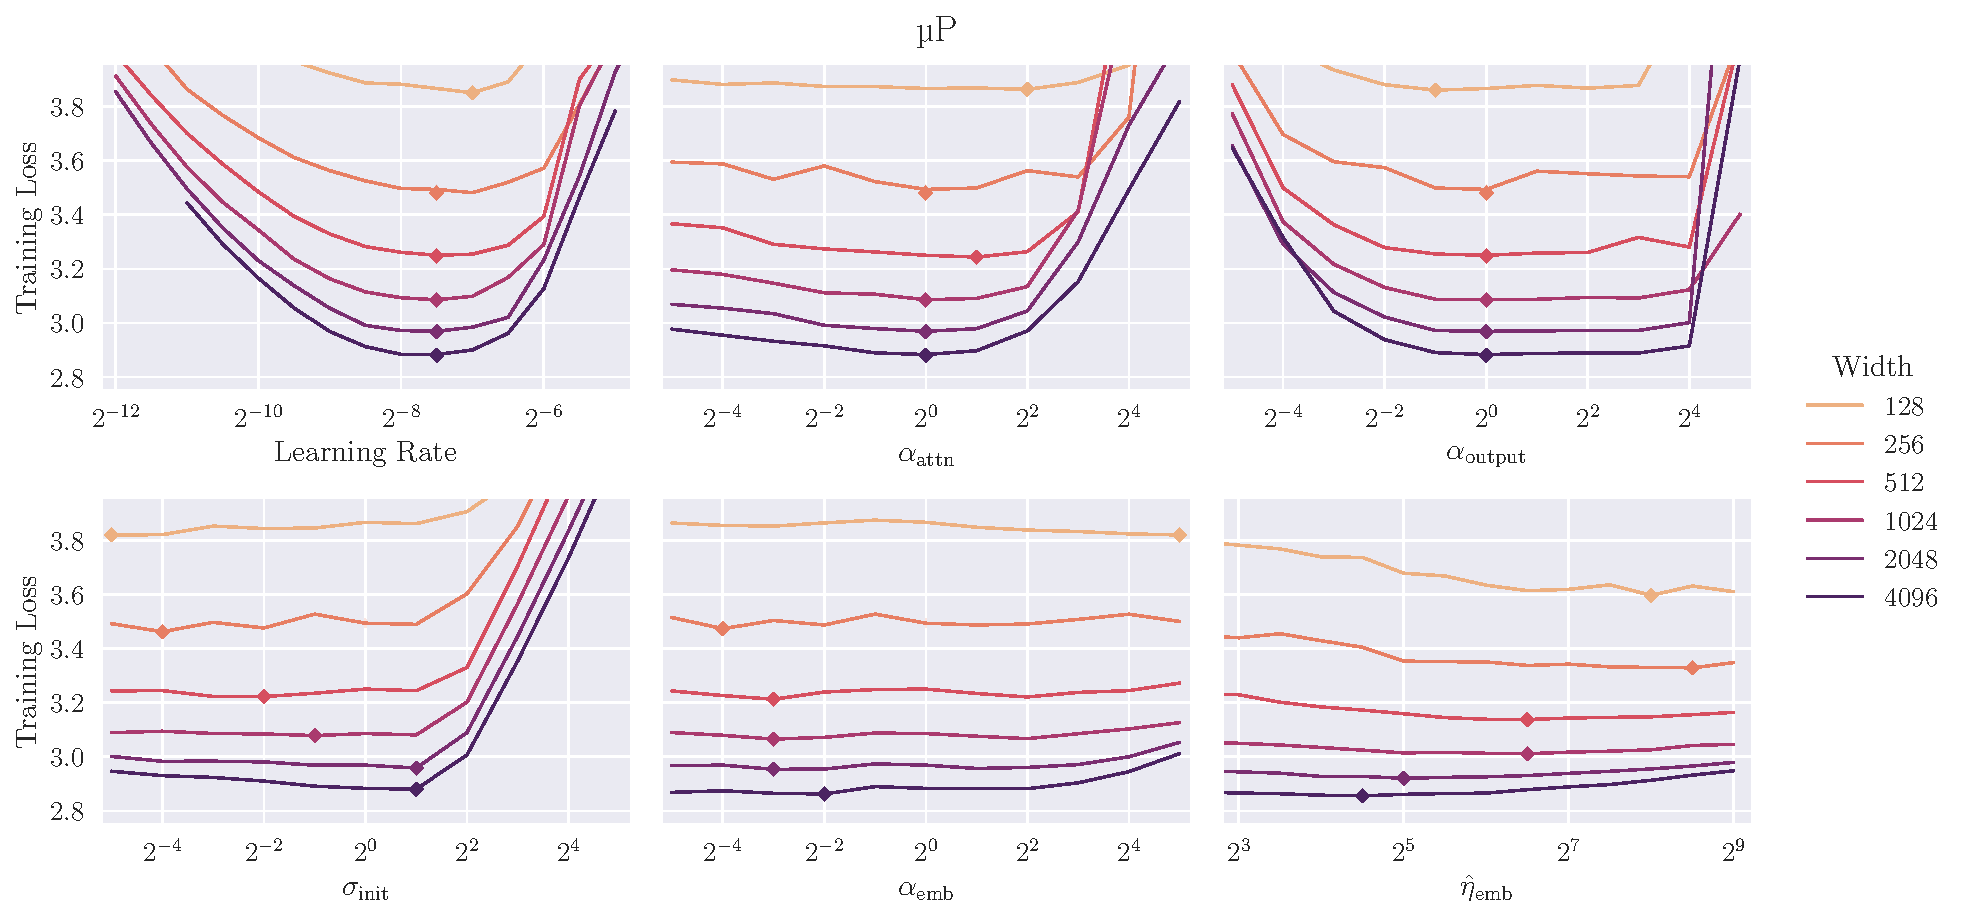
\includegraphics[width=\textwidth]{arXiv/figures/hp_transfer_mup.pdf}
    \vspace{1em}
    \end{subfigure}
    \begin{subfigure}{\textwidth}
        \centering
        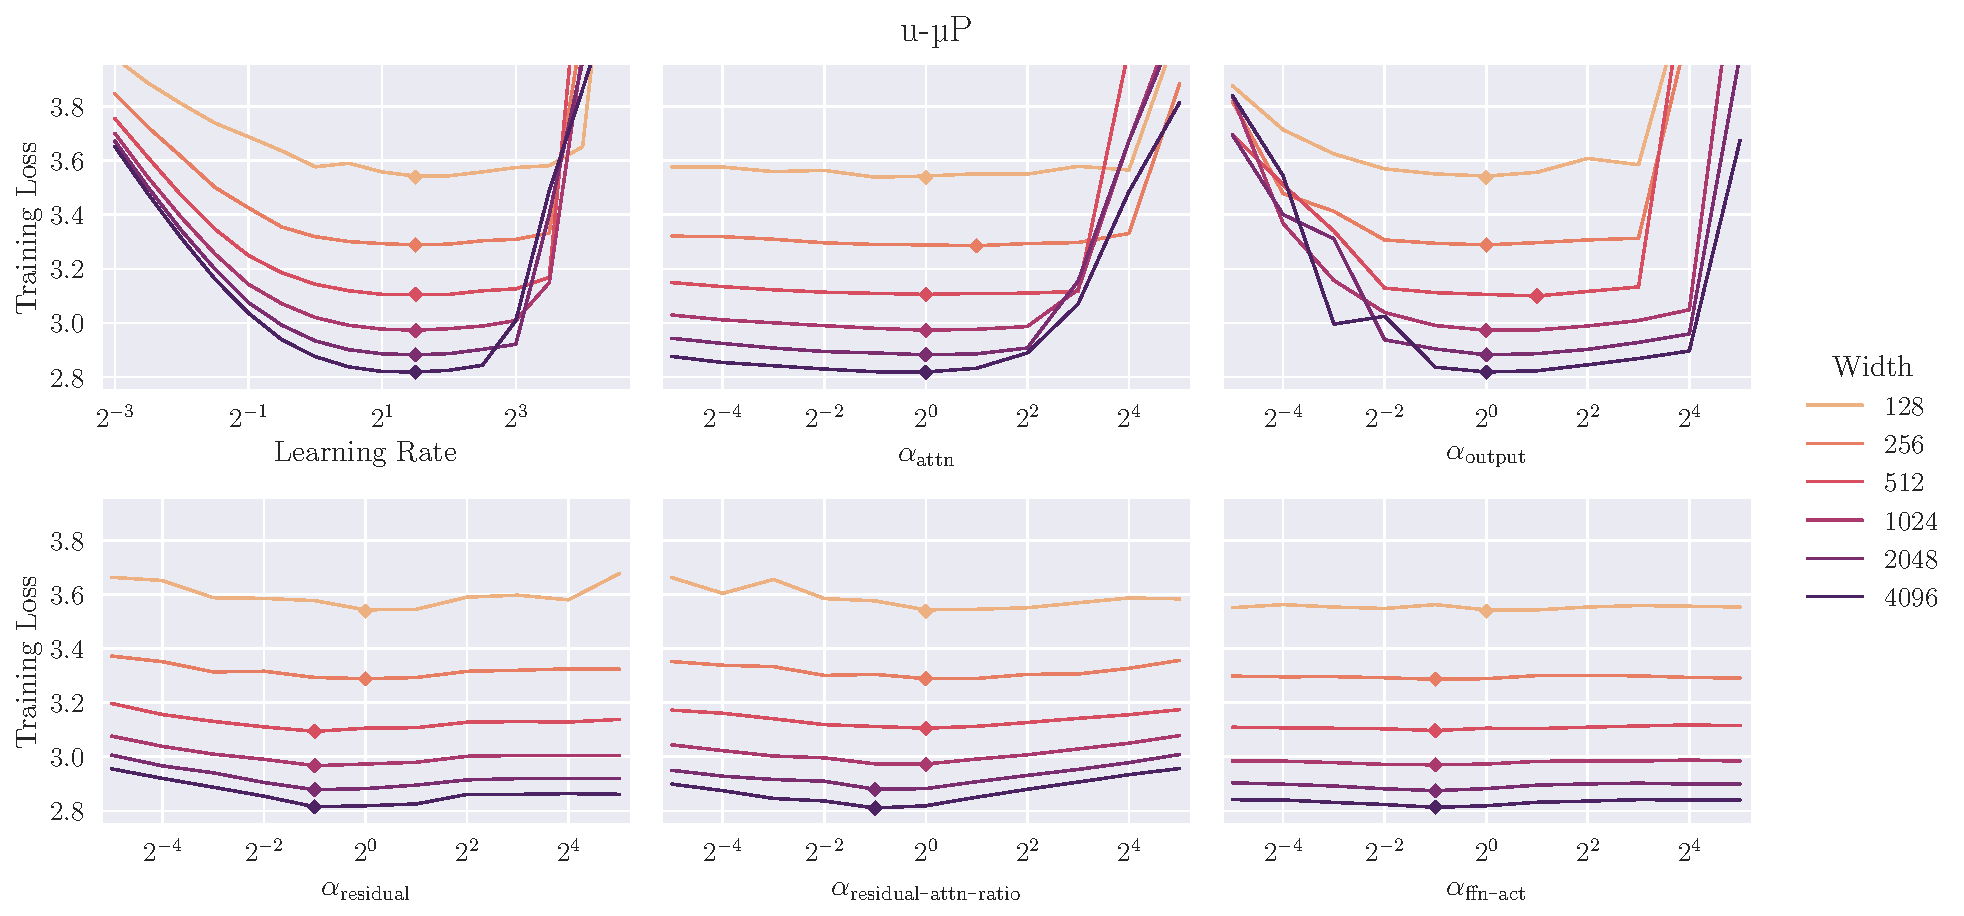
\includegraphics[width=\textwidth]{arXiv/figures/hp_transfer_u-mup.pdf}
    \end{subfigure}
    \caption{Transfer of model hyperparameters over width for \mup{} (top) and \umup{} (bottom). When one hyperparameter is being swept, all others are fixed at $1$, with the exception of Learning Rate $\eta=(2^{1.5}, 2^{-7.5})$ for (\umup{}, \mup{}).}
    \label{fig:experiments:hp_transfer_over_width}
\end{figure}

\paragraph{Combined HP transfer}
Whilst \Cref{fig:experiments:hp_transfer_over_width} demonstrates the transfer of individual hyperparameters over width, \Cref{fig:experiments:SP} instead demonstrates the simultaneous transfer of all hyperparameters when co-optimized on the small-scale proxy model, as is done for \mut. The \mup\ and \umup\ points are taken from \Cref{fig:fig1}, with hyperparameters swept on a model of width 256 using a full random HP search and a simple learning rate sweep for \mup\ and \umup\ respectively. The Standard Parametrization scheme, as shown in \Cref{table:hp_sets} requires choosing a learning rate and a weight-initialization scheme. We follow the initialization scheme of Pythia \citep{Pythia}, and transfer learning rate using a heuristic scaling factor of $\nicefrac{\basewidth}{\mathrm{width}}$, as is done in \citep{LLAMA3}.

\begin{figure}[h]
    \centering
    \includegraphics[width=0.5\textwidth]{arXiv/figures/fig_sp_transfer.pdf}
    \caption{Transferring hyperparameters from width 256 up to 4096 using three different hyperparametrization schemes. \mup\ and \umup\ results are as seen in \Cref{fig:fig1}, whilst Standard Parametrization follows the initialization approach of Pythia \citep{Pythia}.}
    \label{fig:experiments:SP}
\end{figure}

\FloatBarrier
\clearpage

\subsection{Numerical properties} \label{app:fp8_training}

Our analysis of the numerical properties of \umup\ focuses on the RMS of tensors that we wish to cast to FP8: linear module input activations, weights and output gradients.
From the RMS training statistics plots in \Cref{fig:numerics:scale} and \Cref{fig:numerics:rms_during_training} we note that

\begin{enumerate}
    \item \mup{} has gradients and weights with low RMS, at risk of FP8 underflow, whereas \umup{} starts with $\mathrm{RMS} \approx 1$.
    \item Many input activations do not grow RMS during training (due to a preceding non-trainable RMSNorm), however the attention out projection and FFN down projection have unconstrained input activations that grow considerably during training.
    \item The decoder weight grows during training. Since it is preceded by a RMSNorm, the model may require scale growth in order to increase the scale of softmax inputs. Other weights grow slightly during training.
    \item Gradients grow quickly but stabilize, except for attention out projection and FFN down projection, whose gradients shrink as the inputs grow.
\end{enumerate}

We also evaluate how RMS growth is affected by model and training hyperparameters in the tensors that showed the highest end-training RMS, shown in \Cref{fig:numerics:scale_scaling}. This shows that the main parameter affecting scale growth is learning rate, with end-training RMS increasing to the right of the optimal LR basin, as training becomes unstable. End-training RMS is remarkably stable as width, depth, training steps and batch size are independently increased.

\begin{figure}[h]
    \centering
    \begin{subfigure}{\textwidth}
        \centering
        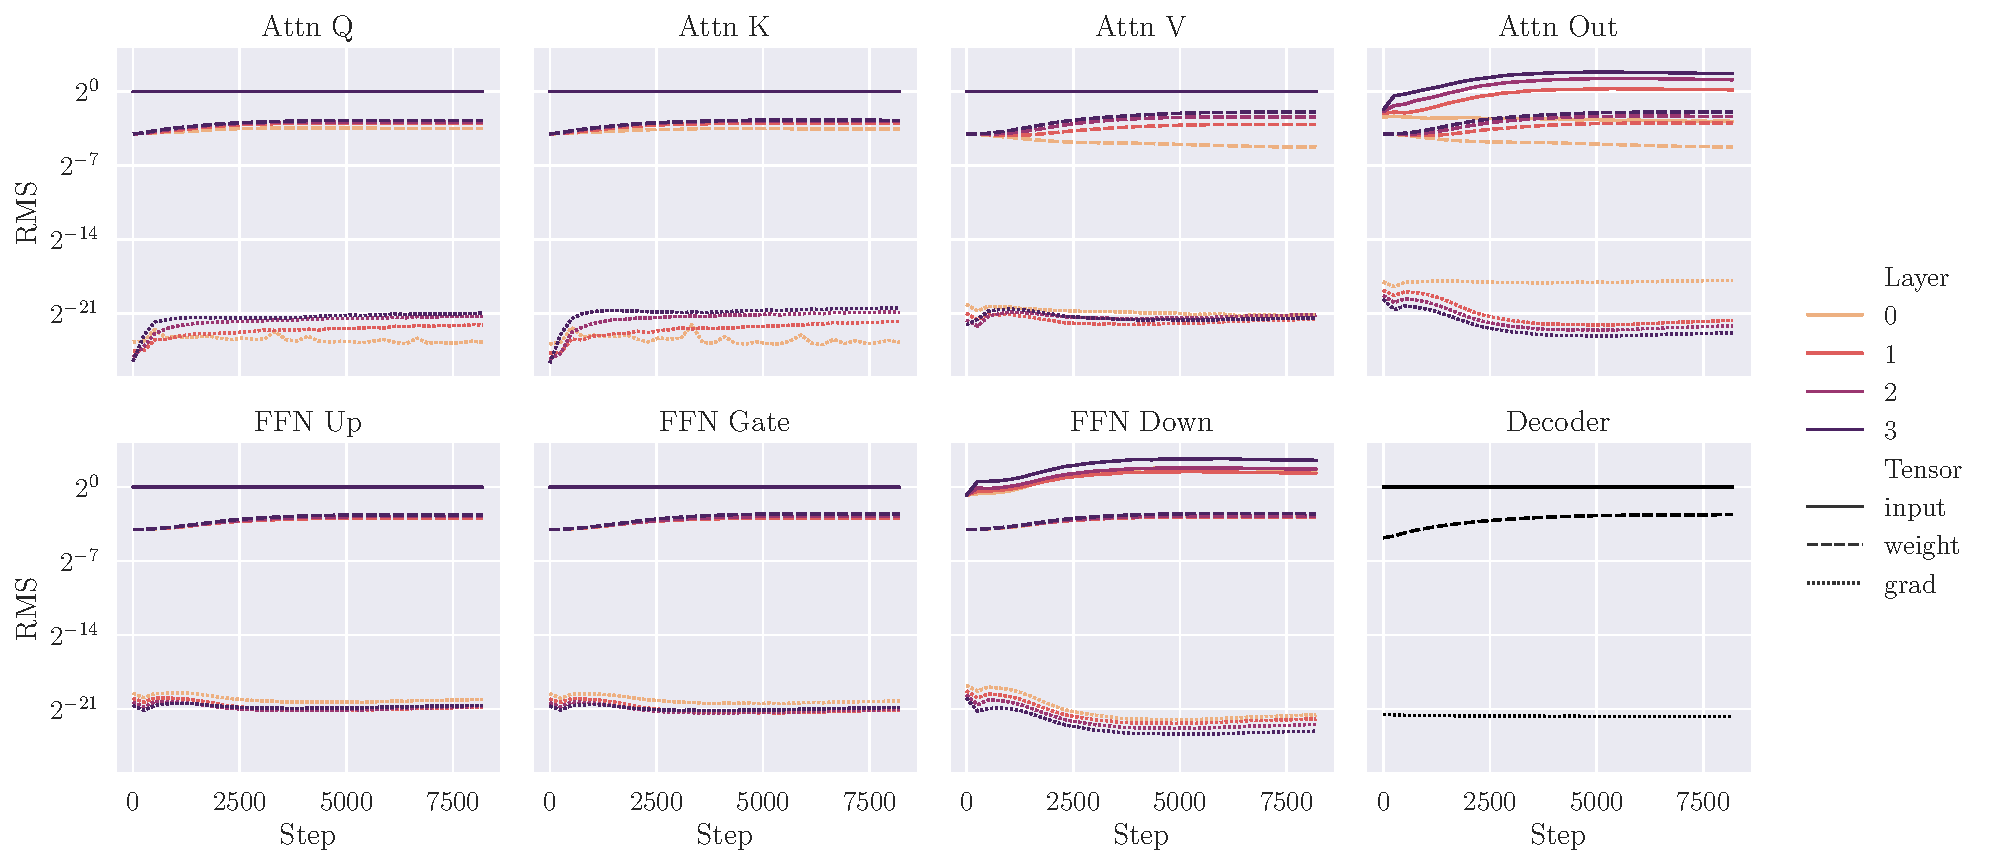
\includegraphics[width=\textwidth]{arXiv/figures/rms_during_training_mup.pdf}
    \end{subfigure}
    \begin{subfigure}{\textwidth}
        \centering
        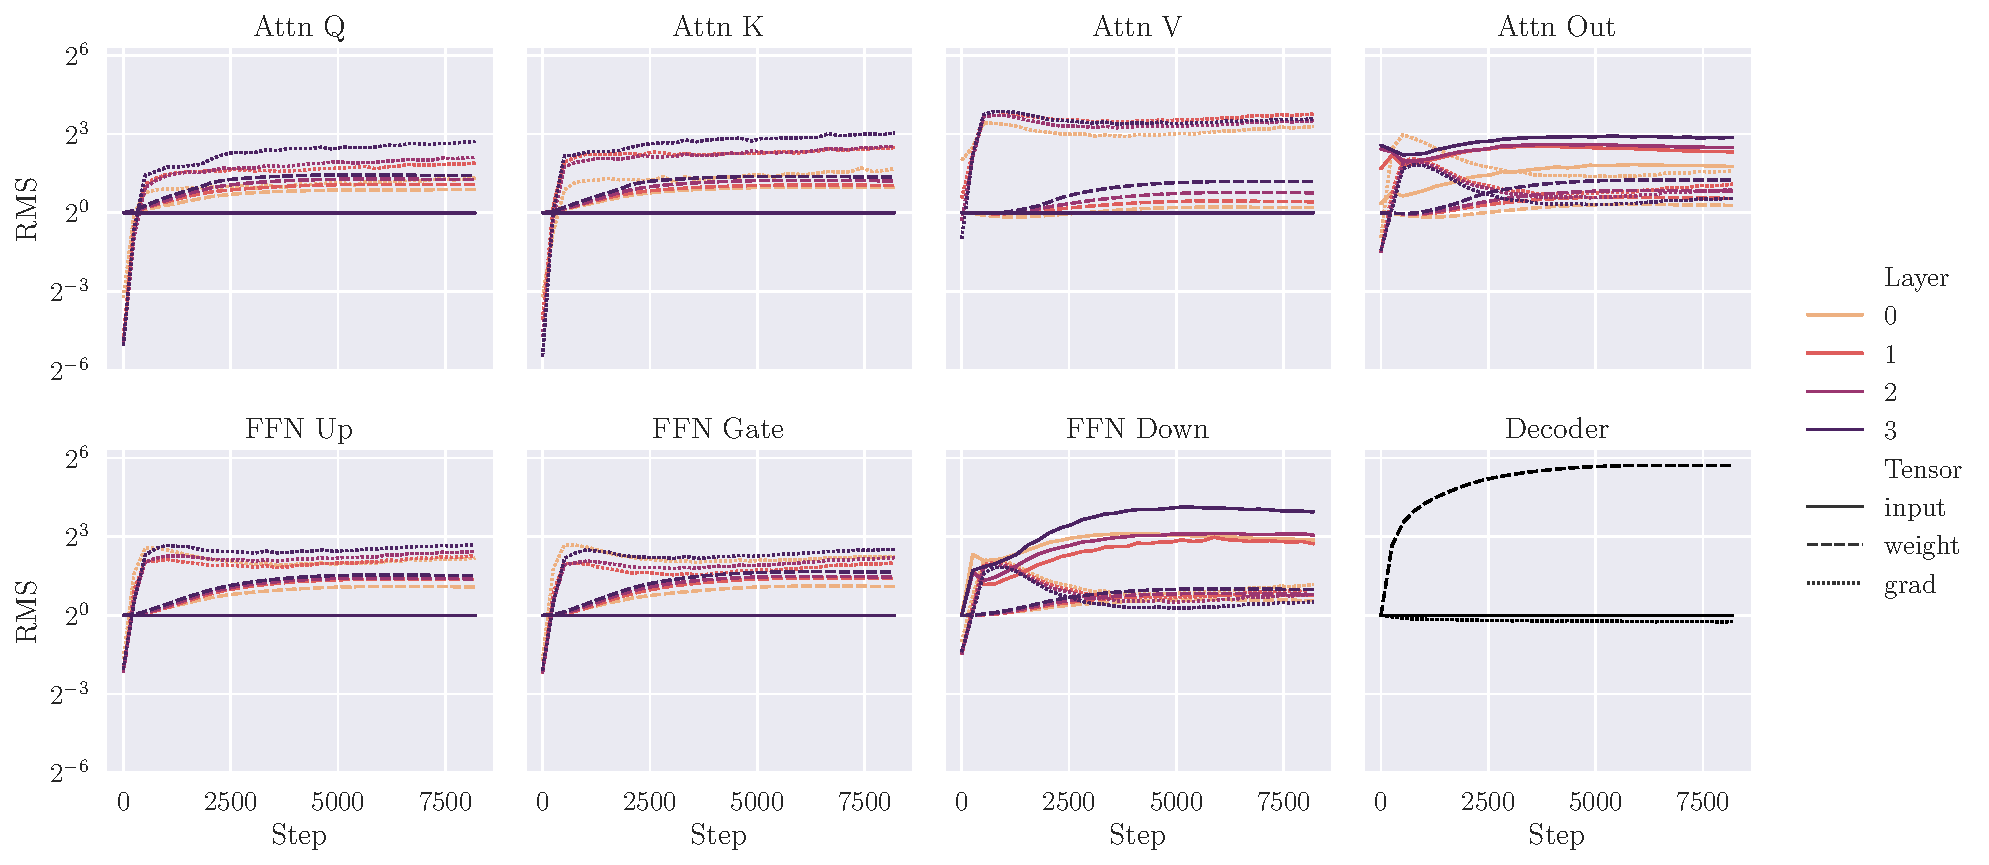
\includegraphics[width=\textwidth]{arXiv/figures/rms_during_training_u-mup.pdf}
    \end{subfigure}
    \caption{RMS during training, for all parametrized matmul inputs, for \mup{} (top) and \umup{} (bottom). Model width $256$, default hyperparameters, $\eta=(2^1, 2^{-8})$ for (\umup{}, \mup{}).}
    \label{fig:numerics:rms_during_training}
\end{figure}

\begin{figure}[h]
    \centering
    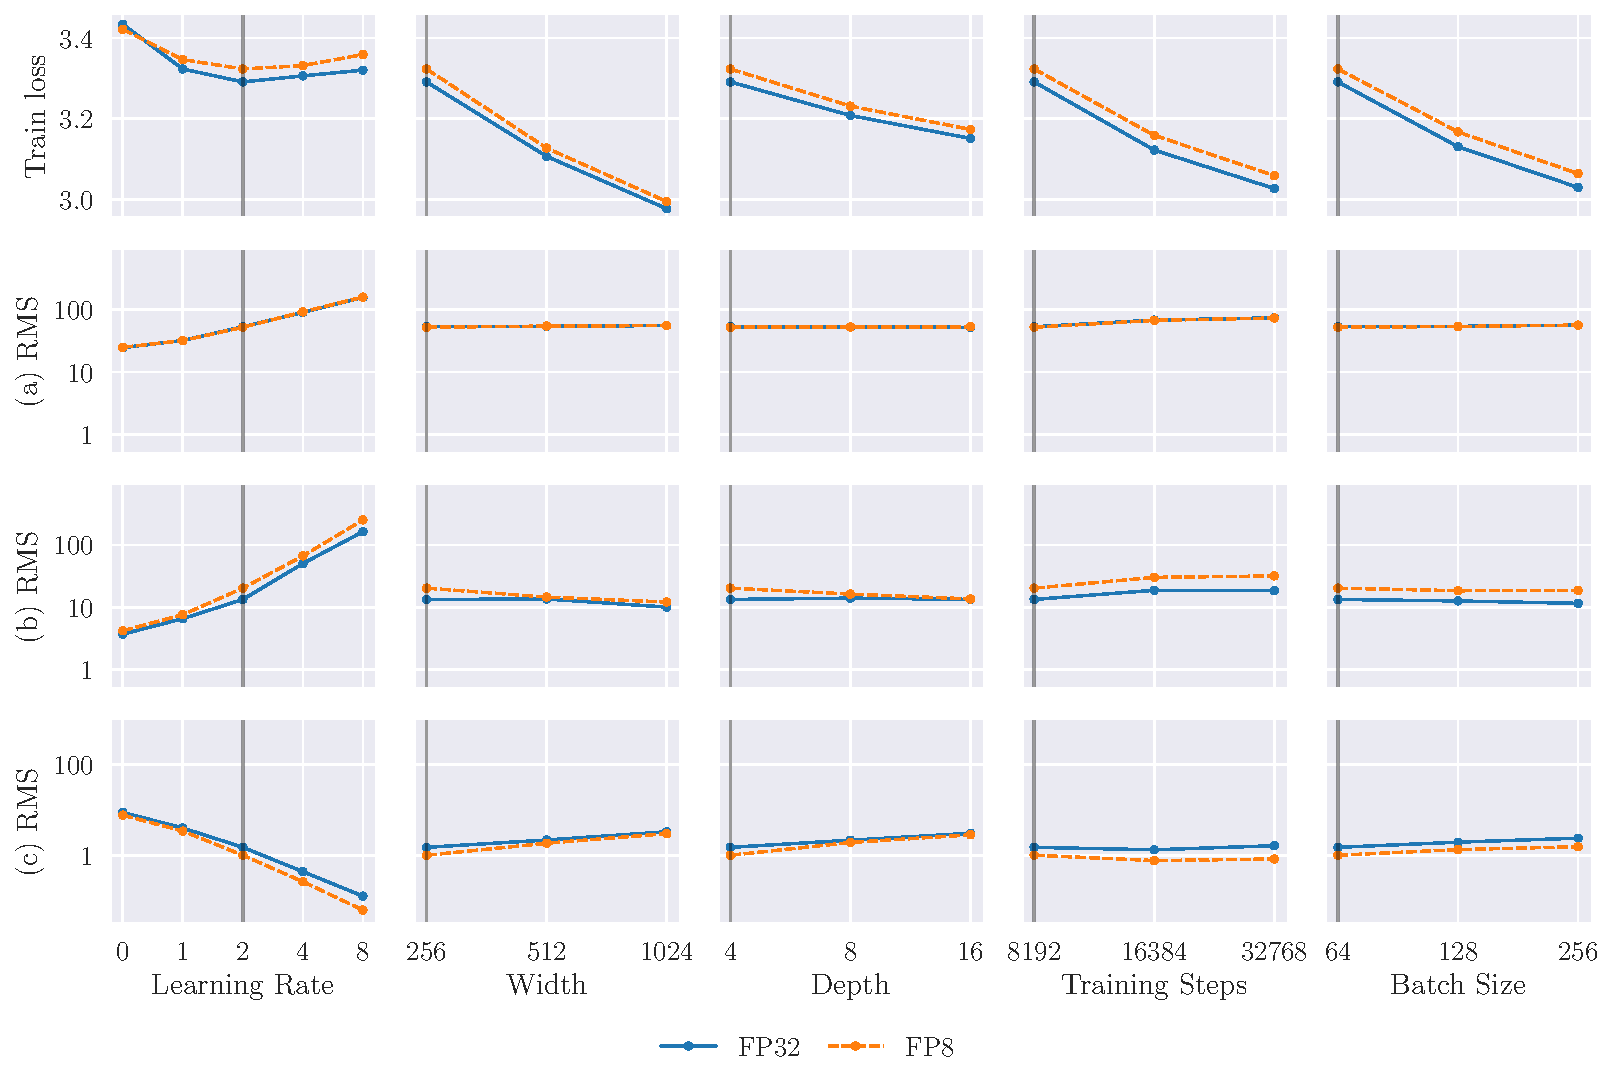
\includegraphics[width=\textwidth]{arXiv/figures/rms_scaling.pdf}
    \caption{The effect of hyperparameters on FP8 training loss and on the end-training RMS of critical tensors: (a) decoder weight, (b) last-layer FFN down-projection input and (c) last-layer FFN down-projection output gradient. Only learning rate has a substantial effect on the end-training RMS. Vertical lines show the default setting of that hyperparameter, as used for all other plots.}
    \label{fig:numerics:scale_scaling}
\end{figure}

%\subsection{Our primary FP8 scheme} \label{app:fp8_scheme}

%Each linear module in a model induces three matrix-matrix products: one during the forward pass to compute the output and two during the backward pass, computing gradients w.r.t.~the weights and the inputs, respectively.
%The tensors participating in these matrix-matrix products are the input activations, the weights and the gradients w.r.t.~the output activations.

%We cast the input, weight and grad-output tensors to the narrower but more accurate \texttt{E4M3} format, and for the two tensors which grow considerably across training---the inputs to FFN and self-attention final projections---we cast to the wider \texttt{E5M2} format. The output of each matrix multiplication is produced directly in the higher-precision format (FP32 in our case), with no loss scaling or per-tensor scaling applied.

%Unit scaling ensures RMS of 1 for all three tensors at initialization, and empirically the scales of these tensors do not drift too much during training, with the exception of the input tensors to the FFN and self-attention final projections, for which we use a wider format due to their increase in RMS over training steps (see \Cref{fig:numerics:rms_during_training}). Note that this scale growth is consistent across different HP settings (see \Cref{fig:numerics:scale_scaling}).

%We have to adapt this scheme slightly for our large-scale training setup, which experiences increased scale-growth for the inputs to FFN and self-attention final projections, exceeding the range of \texttt{E5M2}. Our simple solution to this is a lightweight dynamic re-scaling for those particular problematic operations, still in FP8. This scheme is described in more detail in \Cref{subsec:large_scale}.

\FloatBarrier
\clearpage

% \subsection{FP8 training}

% \begin{figure}[h]
%     \centering
%     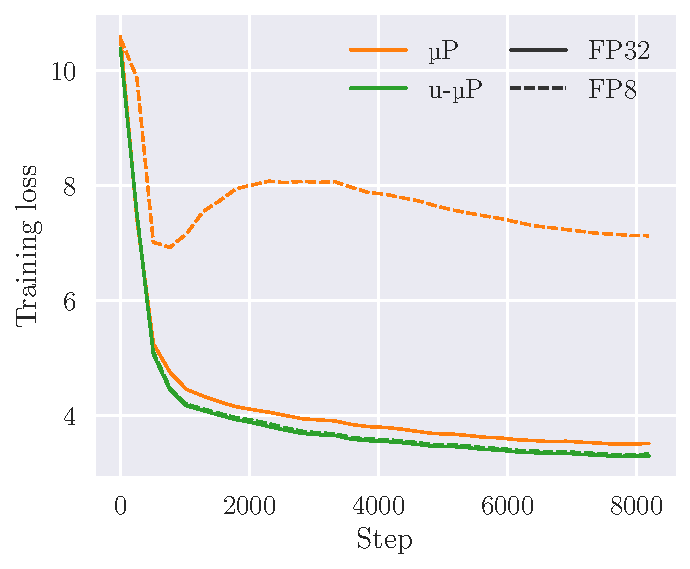
\includegraphics[width=0.47\textwidth]{arXiv/figures/fp8_training_w256.pdf}
%     \caption{FP8 training by direct cast, width $256$, default hyperparameters, $\eta=(2^1, 2^{-8})$ for (\umup{}, \mup{}).}
%     \label{fig:numerics:training_curves}
% \end{figure}

\subsection{Large-scale training details} \label{app:large_model_training}

Our large-scale training settings are given in \Cref{tab:large_scale_experiment_defaults}. These are largely the same as our standard experiments (\Cref{tab:experiment_defaults}), but with many more tokens used for training and scaling up to a larger model-size.
\begin{table}[h] 
    \centering
    \renewcommand{\arraystretch}{1.25}
    \begin{tabular}{|r|p{10cm}|}
    \hline
        Dataset & SlimPajama \citep{SlimPajama} \\
        Sequence length & $4096$ \\
        Vocab size & $65536$ \\
        Training set tokens & $600\mathrm{B}$ \\
        \hline
        Architecture & Llama \citep{Llama} \; (Transformer, PreNorm, RMSNorm, SwiGLU, RoPE, ``untied'' embeddings), non-trainable RMSNorm parameters. \\
        Width & $[2048, 3072, 4096]$ \; (1024 for proxy model) \\
        Depth & $[16, 24, 32]$ \; (8 for proxy model) \\
        Number of heads & $[16, 24, 32]$ \; (8 for proxy model) \\
        % Head-to-layer-ratio & $1$ ($16$ heads, $24$ heads, $32$ heads corresponding to $\sim1,3,7$ B parameters)\\
        Head dimension & $128$ \\
        Total parameters & $[1.07\mathrm{B}, 3.12\mathrm{B}, 6.98\mathrm{B}]$\\
        \hline
        Batch size & $1024$ \\
        Training steps & $72000$ \; ($\sim$ 300B tokens; $20000$ for proxy model) \\
        LR schedule & Cosine to $10\%$, $500$ steps warm-up \\
        Optimizer & AdamW $(\beta_1, \beta_2, \epsilon) = (0.9, 0.95, 10^{-8})$ \\
        Weight decay & $2^{-13}$, independent \citep{Independent_WD} \\
        Dropout & $0.0$ \\
    \hline
    \end{tabular}
    \caption{Large-scale training settings.}
    \label{tab:large_scale_experiment_defaults}
\end{table}

We use mixed-precision during training with optimizer states in FP32 that are sharded via ZeRO stage 1 \citep{Zero}. We retain the model weights in BF16 and apply our FP8 scheme as described in \Cref{sec:umup:low_prec_training} to the tensors participating in matmul operations throughout the transformer block. All other tensors remain either in BF16 (embedding, readout layer, norm, activation function) or FP32 (Flash Attention \citep{Flash_Attention}).

%\begin{itemize}
  %   \item In all matrix multiplications in the transformer block, we use \texttt{E4M3} for the activation and the weight and \texttt{E5M2} for the output gradient.
   %  \item For the attention dense projection and the FFN out projection we use dynamic rescaling as described in Section~\ref{subsec:large_scale}.
     %\item In all remaining matrix multiplications we perform a simple FP8 cast with the aforementioned data types.
%\end{itemize}

Each model was trained on several Nvidia A100 (80GB) or H100 GPUs, with all FP8 experiments conducted on the H100 chips utilizing their native FP8 support. For the FP8 operations we use PyTorch's \texttt{torch.\_scaled\_mm} function as a backbone. 


\FloatBarrier
\clearpage